\documentclass[11pt]{article}

\usepackage[margin=1in]{geometry}
\usepackage[T1]{fontenc}
\usepackage{lmodern}
\usepackage{microtype}
\usepackage{amsmath}
\usepackage{booktabs}
\usepackage{xcolor}
\usepackage{pgfplots}
\pgfplotsset{compat=1.17}
\usepackage[numbers,sort&compress]{natbib}
\usepackage[colorlinks=true,linkcolor=blue!50!black,citecolor=blue!50!black,urlcolor=blue!50!black]{hyperref}

% SOURCE OF TRUTH RULE: no evaluation number is typed in this file.
%   numbers.tex         generated by report/make_numbers.py from results/modal/
%   numbers_manual.tex  hand-kept E1/E2 numbers, each with its source file
% A red ?? in the PDF means the result file is missing. Never replace it by hand.
% GENERATED by report/make_numbers.py. Do not edit by hand.
% source: results/modal
\newcommand{\ExLB}{0.768}
\newcommand{\ExLR}{0.794}
\newcommand{\ExOfficialLB}{0.507}
\newcommand{\ExOfficialLR}{0.520}
\newcommand{\ExOfficialSB}{0.419}
\newcommand{\ExOfficialSR}{0.492}
\newcommand{\ExPctLB}{76.8}
\newcommand{\ExPctLR}{79.4}
\newcommand{\ExPctSB}{59.1}
\newcommand{\ExPctSR}{71.8}
\newcommand{\ExSB}{0.591}
\newcommand{\ExSR}{0.718}
\newcommand{\GapLB}{7.3}
\newcommand{\GapLR}{6.4}
\newcommand{\GapSB}{8.1}
\newcommand{\GapSR}{8.6}
\newcommand{\HeadL}{6.8}
\newcommand{\HeadS}{18.8}
\newcommand{\PassEightLB}{0.797}
\newcommand{\PassEightLR}{0.816}
\newcommand{\PassEightSB}{0.753}
\newcommand{\PassEightSR}{0.786}
\newcommand{\PassOneLB}{0.729}
\newcommand{\PassOneLR}{0.755}
\newcommand{\PassOneSB}{0.566}
\newcommand{\PassOneSR}{0.689}
\newcommand{\SetOpLB}{0.700}
\newcommand{\SetOpLR}{0.675}
\newcommand{\SetOpSB}{0.350}
\newcommand{\SetOpSR}{0.588}
\newcommand{\TsSuiteLB}{0.695}
\newcommand{\TsSuiteLR}{0.730}
\newcommand{\TsSuiteSB}{0.510}
\newcommand{\TsSuiteSR}{0.632}
\newcommand{\dExL}{$+2.6$}
\newcommand{\dExOfficialL}{$+1.3$}
\newcommand{\dExOfficialS}{$+7.3$}
\newcommand{\dExS}{$+12.7$}
\newcommand{\dGapL}{$-0.9$}
\newcommand{\dGapS}{$+0.5$}
\newcommand{\dPassEightL}{$+1.9$}
\newcommand{\dPassEightS}{$+3.3$}
\newcommand{\dPassOneL}{$+2.6$}
\newcommand{\dPassOneS}{$+12.3$}
\newcommand{\dSetOpL}{$-2.5$}
\newcommand{\dSetOpS}{$+23.8$}
\newcommand{\dTsSuiteL}{$+3.5$}
\newcommand{\dTsSuiteS}{$+12.2$}
\newcommand{\SetOpN}{80}
\newcommand{\PlotPassEightLB}{0.797}
\newcommand{\PlotPassEightLR}{0.816}
\newcommand{\PlotPassEightSB}{0.753}
\newcommand{\PlotPassEightSR}{0.786}
\newcommand{\PlotPassOneLB}{0.729}
\newcommand{\PlotPassOneLR}{0.755}
\newcommand{\PlotPassOneSB}{0.566}
\newcommand{\PlotPassOneSR}{0.689}
\newcommand{\EthreeSBDefGEx}{0.418}
\newcommand{\EthreeSBDefGTs}{0.591}
\newcommand{\EthreeSBDefGSuite}{0.510}
\newcommand{\EthreeSBDefGAlias}{2.65}
\newcommand{\EthreeSBDefGQual}{0.45}
\newcommand{\EthreeSBDefVEx}{0.464}
\newcommand{\EthreeSBDefVTs}{0.697}
\newcommand{\EthreeSBDefVSuite}{0.597}
\newcommand{\EthreeSBDefVAlias}{2.21}
\newcommand{\EthreeSBDefVQual}{0.69}
\newcommand{\EthreeSBNoGEx}{0.426}
\newcommand{\EthreeSBNoGTs}{0.585}
\newcommand{\EthreeSBNoGSuite}{0.515}
\newcommand{\EthreeSBNoGAlias}{2.43}
\newcommand{\EthreeSBNoGQual}{0.45}
\newcommand{\EthreeSBNoVEx}{0.511}
\newcommand{\EthreeSBNoVTs}{0.712}
\newcommand{\EthreeSBNoVSuite}{0.607}
\newcommand{\EthreeSBNoVAlias}{1.74}
\newcommand{\EthreeSBNoVQual}{0.87}
\newcommand{\EthreeSBAlGEx}{0.224}
\newcommand{\EthreeSBAlGTs}{0.432}
\newcommand{\EthreeSBAlGSuite}{0.366}
\newcommand{\EthreeSBAlGAlias}{6.28}
\newcommand{\EthreeSBAlGQual}{0.00}
\newcommand{\EthreeSBAlVEx}{0.347}
\newcommand{\EthreeSBAlVTs}{0.617}
\newcommand{\EthreeSBAlVSuite}{0.502}
\newcommand{\EthreeSBAlVAlias}{5.87}
\newcommand{\EthreeSBAlVQual}{0.02}
\newcommand{\EthreeSRDefGEx}{0.489}
\newcommand{\EthreeSRDefGTs}{0.714}
\newcommand{\EthreeSRDefGSuite}{0.629}
\newcommand{\EthreeSRDefGAlias}{0.37}
\newcommand{\EthreeSRDefGQual}{1.40}
\newcommand{\EthreeSRDefVEx}{0.499}
\newcommand{\EthreeSRDefVTs}{0.744}
\newcommand{\EthreeSRDefVSuite}{0.641}
\newcommand{\EthreeSRDefVAlias}{0.36}
\newcommand{\EthreeSRDefVQual}{1.45}
\newcommand{\EthreeSRNoGEx}{0.502}
\newcommand{\EthreeSRNoGTs}{0.730}
\newcommand{\EthreeSRNoGSuite}{0.636}
\newcommand{\EthreeSRNoGAlias}{0.31}
\newcommand{\EthreeSRNoGQual}{1.44}
\newcommand{\EthreeSRNoVEx}{0.526}
\newcommand{\EthreeSRNoVTs}{0.746}
\newcommand{\EthreeSRNoVSuite}{0.656}
\newcommand{\EthreeSRNoVAlias}{0.35}
\newcommand{\EthreeSRNoVQual}{1.45}
\newcommand{\EthreeSRAlGEx}{0.420}
\newcommand{\EthreeSRAlGTs}{0.627}
\newcommand{\EthreeSRAlGSuite}{0.566}
\newcommand{\EthreeSRAlGAlias}{5.48}
\newcommand{\EthreeSRAlGQual}{0.01}
\newcommand{\EthreeSRAlVEx}{0.467}
\newcommand{\EthreeSRAlVTs}{0.709}
\newcommand{\EthreeSRAlVSuite}{0.626}
\newcommand{\EthreeSRAlVAlias}{5.27}
\newcommand{\EthreeSRAlVQual}{0.02}
\newcommand{\EthreeVoteShareTs}{86}
\newcommand{\EthreeVoteNoShareTs}{98}
\newcommand{\dEthreeAlSBTs}{$-15.9$}
\newcommand{\dEthreeNoSBTs}{$-0.6$}
\newcommand{\dEthreeVoteSBTs}{$+10.6$}
\newcommand{\dEthreeAlSRTs}{$-8.7$}
\newcommand{\dEthreeNoSRTs}{$+1.6$}
\newcommand{\dEthreeVoteSRTs}{$+3.0$}
\newcommand{\EthreeVoteShareSuite}{73}
\newcommand{\EthreeVoteNoShareSuite}{82}
\newcommand{\dEthreeAlSBSuite}{$-14.4$}
\newcommand{\dEthreeNoSBSuite}{$+0.5$}
\newcommand{\dEthreeVoteSBSuite}{$+8.7$}
\newcommand{\dEthreeAlSRSuite}{$-6.3$}
\newcommand{\dEthreeNoSRSuite}{$+0.7$}
\newcommand{\dEthreeVoteSRSuite}{$+1.2$}
\newcommand{\EthreeVoteShareEx}{65}
\newcommand{\EthreeVoteNoShareEx}{131}
\newcommand{\dEthreeAlSBEx}{$-19.4$}
\newcommand{\dEthreeNoSBEx}{$+0.8$}
\newcommand{\dEthreeVoteSBEx}{$+4.6$}
\newcommand{\dEthreeAlSREx}{$-6.9$}
\newcommand{\dEthreeNoSREx}{$+1.3$}
\newcommand{\dEthreeVoteSREx}{$+1.0$}
\newcommand{\EfourBaseEx}{0.424}
\newcommand{\EfourBaseTs}{0.592}
\newcommand{\EfourBaseSuite}{0.511}
\newcommand{\EfourBaseValid}{0.784}
\newcommand{\EfourBaseAlias}{2.62}
\newcommand{\EfourBaseQual}{0.45}
\newcommand{\EfourGrpoEx}{0.492}
\newcommand{\EfourGrpoTs}{0.720}
\newcommand{\EfourGrpoSuite}{0.633}
\newcommand{\EfourGrpoValid}{0.910}
\newcommand{\EfourGrpoAlias}{0.34}
\newcommand{\EfourGrpoQual}{1.41}
\newcommand{\EfourTopTwoHalfEx}{0.306}
\newcommand{\EfourTopTwoHalfTs}{0.463}
\newcommand{\EfourTopTwoHalfSuite}{0.394}
\newcommand{\EfourTopTwoHalfValid}{0.633}
\newcommand{\EfourTopTwoHalfAlias}{0.00}
\newcommand{\EfourTopTwoHalfQual}{1.93}
\newcommand{\EfourTopTwoOneEx}{0.000}
\newcommand{\EfourTopTwoOneTs}{0.000}
\newcommand{\EfourTopTwoOneSuite}{0.000}
\newcommand{\EfourTopTwoOneValid}{0.000}
\newcommand{\EfourTopTwoOneAlias}{0.00}
\newcommand{\EfourTopTwoOneQual}{0.00}
\newcommand{\EfourTopEightQuarterEx}{0.116}
\newcommand{\EfourTopEightQuarterTs}{0.137}
\newcommand{\EfourTopEightQuarterSuite}{0.133}
\newcommand{\EfourTopEightQuarterValid}{0.165}
\newcommand{\EfourTopEightQuarterAlias}{0.00}
\newcommand{\EfourTopEightQuarterQual}{0.50}
\newcommand{\EfourTopEightHalfEx}{0.000}
\newcommand{\EfourTopEightHalfTs}{0.000}
\newcommand{\EfourTopEightHalfSuite}{0.000}
\newcommand{\EfourTopEightHalfValid}{0.000}
\newcommand{\EfourTopEightHalfAlias}{0.00}
\newcommand{\EfourTopEightHalfQual}{0.00}
\newcommand{\EfourRandTwoOneEx}{0.000}
\newcommand{\EfourRandTwoOneTs}{0.000}
\newcommand{\EfourRandTwoOneSuite}{0.000}
\newcommand{\EfourRandTwoOneValid}{0.000}
\newcommand{\EfourRandTwoOneAlias}{0.00}
\newcommand{\EfourRandTwoOneQual}{0.00}
\newcommand{\EfourRandEightHalfEx}{0.000}
\newcommand{\EfourRandEightHalfTs}{0.000}
\newcommand{\EfourRandEightHalfSuite}{0.000}
\newcommand{\EfourRandEightHalfValid}{0.000}
\newcommand{\EfourRandEightHalfAlias}{0.00}
\newcommand{\EfourRandEightHalfQual}{0.00}
\newcommand{\EfourZeroEightEx}{0.433}
\newcommand{\EfourZeroEightTs}{0.620}
\newcommand{\EfourZeroEightSuite}{0.541}
\newcommand{\EfourZeroEightValid}{0.811}
\newcommand{\EfourZeroEightAlias}{1.32}
\newcommand{\EfourZeroEightQual}{1.00}
\newcommand{\EfourTopTwoOneRevEx}{0.000}
\newcommand{\EfourTopTwoOneRevTs}{0.000}
\newcommand{\EfourTopTwoOneRevSuite}{0.000}
\newcommand{\EfourTopTwoOneRevValid}{0.000}
\newcommand{\EfourTopTwoOneRevAlias}{0.00}
\newcommand{\EfourTopTwoOneRevQual}{0.00}
\newcommand{\EfourGrpoTopTwoOneRevEx}{0.000}
\newcommand{\EfourGrpoTopTwoOneRevTs}{0.000}
\newcommand{\EfourGrpoTopTwoOneRevSuite}{0.000}
\newcommand{\EfourGrpoTopTwoOneRevValid}{0.000}
\newcommand{\EfourGrpoTopTwoOneRevAlias}{0.00}
\newcommand{\EfourGrpoTopTwoOneRevQual}{0.00}
\newcommand{\EfourZeroShareTs}{22}
\newcommand{\EfourZeroShareSuite}{25}
\newcommand{\dEfourZeroTs}{$+2.8$}
\newcommand{\dEfourZeroSuite}{$+3.0$}
\newcommand{\dEfourTopTwoHalfTs}{$-12.9$}
\newcommand{\dEfourTopTwoHalfSuite}{$-11.7$}
\newcommand{\EfourSteered}{8}
\newcommand{\EfourBroken}{6}
\newcommand{\EfourPairs}{139}
\newcommand{\EfourScreenPairs}{32}
\newcommand{\EfourMBase}{-5.36}
\newcommand{\EfourMRl}{-11.07}
\newcommand{\EfourDm}{-5.72}
\newcommand{\EfourAtpTotal}{-7.48}
\newcommand{\EfourPrefAliasBase}{5.0}
\newcommand{\EfourPrefAliasRl}{0.7}
\newcommand{\EfourTopShare}{10}
\newcommand{\EfourTopN}{50}
\newcommand{\EfourTopLayer}{27}
\newcommand{\EfourTopLayerCount}{17}
\newcommand{\EfourScreened}{40}
\newcommand{\EfourAgree}{21}
\newcommand{\EfourScrALayer}{27}
\newcommand{\EfourScrANeuron}{3289}
\newcommand{\EfourScrAAtpRank}{5}
\newcommand{\EfourScrBLayer}{27}
\newcommand{\EfourScrBNeuron}{2651}
\newcommand{\EfourScrBAtpRank}{210}

% Hand-maintained numbers that make_numbers.py does not read yet.
% Every line names its source file. Change a value only after opening that file.

% E1, results/modal/e1/{1.5b,7b}_summary.json
\newcommand{\KLS}{0.043}          % mean per-token KL, 1.5B base vs GRPO, nats
\newcommand{\KLL}{0.012}          % same, 7B
\newcommand{\KLRatio}{3.65}       % KLS / KLL as reported by E1
\newcommand{\FixedS}{155}         % dev questions wrong before, right after (E1 checker)
\newcommand{\FixedL}{35}
\newcommand{\EntS}{0.11}          % 1.5B mean entropy drop, nats
\newcommand{\ConcAggL}{17.3}      % 7B: KL share at aggregate tokens / token share, FIXED questions
\newcommand{\ConcFromL}{5.2}      % 7B: same, FROM-clause tokens

% E2, results/modal/e2/{1.5b,7b}_summary.json  (per query, Spider dev)
\newcommand{\AliasGold}{2.93}
\newcommand{\AliasSB}{2.63}
\newcommand{\AliasSR}{0.36}
\newcommand{\AliasLB}{0.43}
\newcommand{\AliasLR}{0.45}
\newcommand{\QualSB}{0.46}
\newcommand{\QualSR}{1.41}
\newcommand{\QualLB}{1.62}
\newcommand{\QualLR}{1.59}
\newcommand{\JoinSB}{0.51}
\newcommand{\JoinSR}{0.35}
\newcommand{\EceSB}{0.049}
\newcommand{\EceSR}{0.062}
\newcommand{\EceLB}{0.074}
\newcommand{\EceLR}{0.086}

% Training logs, W&B / results/grpo_7k_trainlog.json
\newcommand{\ZeroStd}{0.625}      % mean frac_reward_zero_std


\newcommand{\todo}[1]{\textcolor{red}{[TODO: #1]}}
\newcommand{\pp}{\,pp}

\title{Sharpening Where There Is Headroom:\\
What GRPO Changes in Text-to-SQL Across Model Scale}
\author{Ved Chadderwala\\
University of Southern California\\
\texttt{chadderw@usc.edu}}
\date{Working draft, \today \\ \small Code and results: \url{https://github.com/ved-2004/RLVR-Text-to-SQL}}

\begin{document}
\maketitle

%==========================================================================
\section{Introduction and Motivation}
%==========================================================================

Reinforcement learning from verifiable rewards (RLVR) has become a standard
post-training step for reasoning and code models
\citep{shao2024deepseekmath,lambert2024tulu3,guo2025deepseekr1}. The recipe is
simple: sample several answers, check each with a program, and push the model
toward the ones that pass. What is less clear is \emph{what} this changes. A
model that gets more questions right after RL could have learned to solve new
problems, or it could have learned to pick, on the first try, an answer it was
already able to produce some of the time. \citet{yue2025limit} argue that on
math and code benchmarks it is mostly the second: RL raises pass@1 but does not
raise, and can lower, pass@$k$ for large $k$.

This report studies that question on text-to-SQL, which is a useful instrument
for three reasons. First, the verifier is cheap and objective: execute the
query and compare result sets. Second, the verifier has a known and measurable
false-positive rate, because a wrong query can return the right rows on one
database by coincidence \citep{zhong2020testsuite}. This lets us check whether
the policy learns to exploit the reward. Third, SQL tokens carry explicit roles
(keywords, aggregates, table names, aliases, literals), so token-level changes
can be grouped by what they do.

We train Qwen2.5-Coder-Instruct at 1.5B and 7B parameters \citep{hui2024qwen25coder}
with one fixed GRPO recipe and a binary execution reward on the Spider training
set \citep{yu2018spider}, then ask four questions:
\begin{enumerate}
  \item How much does the same recipe help at each scale, and what predicts the size of the gain?
  \item Where in the output distribution does the model move, and does that differ by scale?
  \item Does RL change \emph{how} the model writes SQL, not only whether it is correct?
  \item Does the policy learn to exploit the verifier's false positives?
\end{enumerate}

Our main findings are:
\begin{itemize}
  \item The same recipe raises execution accuracy by \dExS\pp{} at 1.5B
        (\ExPctSB\% to \ExPctSR\%) and by \dExL\pp{} at 7B (\ExPctLB\% to \ExPctLR\%).
        The size of the gain lines up with the base model's pass@1 to pass@8 gap
        (\HeadS{} vs.\ \HeadL{} points). This is a two-point observation, not a fitted law.
  \item The 1.5B model moves $\KLRatio\times$ further from its base in per-token KL and
        fixes \FixedS{} dev questions versus \FixedL{} for the 7B. The 1.5B change is broad;
        the 7B change is concentrated on aggregate and \texttt{FROM}-clause tokens.
  \item Without any style term in the reward, the 1.5B model drops table aliases
        (\AliasSB{} to \AliasSR{} per query) and switches to \texttt{table.column} references,
        which is how the untrained 7B already writes. It moves \emph{away} from the
        style of the gold queries.
  \item The single-database vs.\ test-suite gap stays between 6 and 9 points.
        It narrows at 7B and widens slightly at 1.5B, so we see no clear sign of
        reward hacking, but also no sign that RL removes the false positives.
\end{itemize}

%==========================================================================
\section{Background and Related Work}
%==========================================================================

\paragraph{GRPO and RLVR.}
Group Relative Policy Optimization \citep{shao2024deepseekmath} drops the value
network of PPO. For each prompt it samples a group of $G$ completions, scores
them, and uses the group-normalized reward as the advantage:
\begin{equation}
  \hat{A}_i = \frac{r_i - \operatorname{mean}(r_1,\dots,r_G)}{\operatorname{std}(r_1,\dots,r_G)} .
\end{equation}
A KL penalty with coefficient $\beta$ keeps the policy near a reference model.
When every completion in a group gets the same reward, all advantages are zero
and the prompt contributes no gradient. DAPO \citep{yu2025dapo} addresses this
with dynamic sampling, which filters out such groups. RLVR with GRPO-style
updates is used in DeepSeek-R1 \citep{guo2025deepseekr1} and T\"ulu~3
\citep{lambert2024tulu3}.

\paragraph{Does RL add capability?}
\citet{yue2025limit} compare base and RL-trained models with pass@$k$
\citep{chen2021codex} at large $k$ and find that base models match or beat RL
models once $k$ is large, which suggests RL mostly reweights solutions already
in the base model's distribution. \citet{mukherjee2025subnetworks} find that RL
updates only a small subnetwork of parameters, consistent with a light-touch
change. Our scale comparison asks a related question from a different side: if
RL mostly converts existing pass@$k$ into pass@1, the room available to convert
should predict the gain.

\paragraph{RL for text-to-SQL.}
SQL-R1 \citep{ma2025sqlr1} trains reasoning models with GRPO and execution-based
rewards. Reasoning-SQL \citep{pourreza2025reasoningsql} adds partial rewards for
schema linking, syntax, and n-gram similarity. Both target state-of-the-art
accuracy. We instead keep the recipe minimal (binary reward, no reasoning
trace, LoRA) so that changes can be attributed and compared across scale.

\paragraph{Evaluating SQL by execution.}
Spider \citep{yu2018spider} reports exact set match and execution accuracy.
Execution accuracy has false positives: a query such as \texttt{WHERE age > 34}
may return the same rows as the gold \texttt{WHERE age >= 34} on one database.
Test-suite accuracy \citep{zhong2020testsuite} runs each query on a distilled
set of perturbed databases and counts it correct only if it matches gold on all
of them. Because our reward is execution on a single database, the gap between
single-database and test-suite accuracy measures how much of the reward is
earned by coincidence.

%==========================================================================
\section{Experiments and Results}
%==========================================================================

\subsection{Setup}

\paragraph{Models.} Qwen2.5-Coder-1.5B-Instruct and Qwen2.5-Coder-7B-Instruct
\citep{hui2024qwen25coder}. These are general code models, not SQL-specialized,
so that a gain from RL is not confounded with prior SQL fine-tuning.

\paragraph{Training.} GRPO via TRL \texttt{GRPOTrainer} with LoRA
\citep{hu2021lora} ($r=16$, $\alpha=32$, all linear layers), $G=8$ completions
per prompt, learning rate $10^{-5}$, $\beta=0.04$, sampling temperature 0.9.
Training data is the full Spider train set (7{,}000 examples).
\todo{epochs, batch size, max completion length, wall-clock and GPU type}.
The prompt gives the schema as one line per table and asks for a single SQLite
query in a \texttt{sql} code block. There is no reasoning trace.

\paragraph{Reward.} Binary execution reward: extract the query, run it read-only
on the example's SQLite database with a 5\,s timeout, and return 1 if its result
set equals the gold result set, else 0. Write statements are rejected.

\paragraph{Evaluation.} Full Spider dev set (1{,}034 questions), greedy decoding
with vLLM, identical prompt for all four models. We report:
\begin{itemize}
  \item \textbf{EX}: execution accuracy from the test-suite evaluator
        \citep{zhong2020testsuite} run on the original dev databases.
  \item \textbf{TS}: the same evaluator run on the distilled test suite. Because
        only the databases change, \textbf{EX $-$ TS} (the FP gap) isolates false positives.
  \item \textbf{EX (official)}: the original Spider evaluator, for comparison.
  \item \textbf{pass@1 / pass@8}: from 8 samples per question, scored with a
        set-based result comparison. \todo{sampling temperature for pass@k}.
  \item \textbf{Set-op EX}: execution accuracy on the \SetOpN{} dev questions whose
        gold query uses \texttt{INTERSECT}, \texttt{UNION} or \texttt{EXCEPT}.
  \item \textbf{ECE}: expected calibration error. \todo{state exactly what confidence is binned}.
\end{itemize}

\paragraph{Evaluation note.} Two earlier versions of these numbers were wrong.
The first pipeline truncated long prompts at 1{,}536 tokens and reported a 1.5B base
EX of 34.5\%. The second saved only the last 2{,}500 characters of the official
evaluator's log, which cut off the execution row; the value we read as EX was the
SELECT-clause partial-match recall. All numbers in this report are generated from
the stored result files by \texttt{report/make\_numbers.py}, which reads each
metric by its row in the evaluator output.

\subsection{Main results}

\begin{table}[h]
\centering
\caption{Spider dev results. $\Delta$ is in percentage points.}
\label{tab:main}
\begin{tabular}{lcccccc}
\toprule
 & \multicolumn{3}{c}{1.5B} & \multicolumn{3}{c}{7B} \\
\cmidrule(lr){2-4}\cmidrule(lr){5-7}
Metric & Base & GRPO & $\Delta$ & Base & GRPO & $\Delta$ \\
\midrule
EX                & \ExSB & \ExSR & \dExS & \ExLB & \ExLR & \dExL \\
TS                & \TsSuiteSB & \TsSuiteSR & \dTsSuiteS & \TsSuiteLB & \TsSuiteLR & \dTsSuiteL \\
FP gap (pts)      & \GapSB & \GapSR & \dGapS & \GapLB & \GapLR & \dGapL \\
EX (official)     & \ExOfficialSB & \ExOfficialSR & \dExOfficialS & \ExOfficialLB & \ExOfficialLR & \dExOfficialL \\
\midrule
pass@1            & \PassOneSB & \PassOneSR & \dPassOneS & \PassOneLB & \PassOneLR & \dPassOneL \\
pass@8            & \PassEightSB & \PassEightSR & \dPassEightS & \PassEightLB & \PassEightLR & \dPassEightL \\
\midrule
Set-op EX         & \SetOpSB & \SetOpSR & \dSetOpS & \SetOpLB & \SetOpLR & \dSetOpL \\
ECE               & \EceSB & \EceSR &  & \EceLB & \EceLR &  \\
\bottomrule
\end{tabular}
\end{table}

GRPO helps the 1.5B model on every execution metric by about 12 to 13 points
and the 7B by about 2 to 3.5 (Table~\ref{tab:main}). The untrained 7B still beats
the trained 1.5B on EX (\ExLB{} vs.\ \ExSR). Calibration gets slightly worse at
both scales.

\subsection{The gain tracks sampling headroom}

\begin{table}[h]
\centering
\caption{Headroom before training vs.\ gain after training (points).}
\label{tab:headroom}
\begin{tabular}{lcccc}
\toprule
Model & pass@8 $-$ pass@1 (base) & $\Delta$ pass@1 & $\Delta$ pass@8 & $\Delta$ EX \\
\midrule
1.5B & \HeadS & \dPassOneS & \dPassEightS & \dExS \\
7B   & \HeadL & \dPassOneL & \dPassEightL & \dExL \\
\bottomrule
\end{tabular}
\end{table}

\begin{figure}[h]
\centering
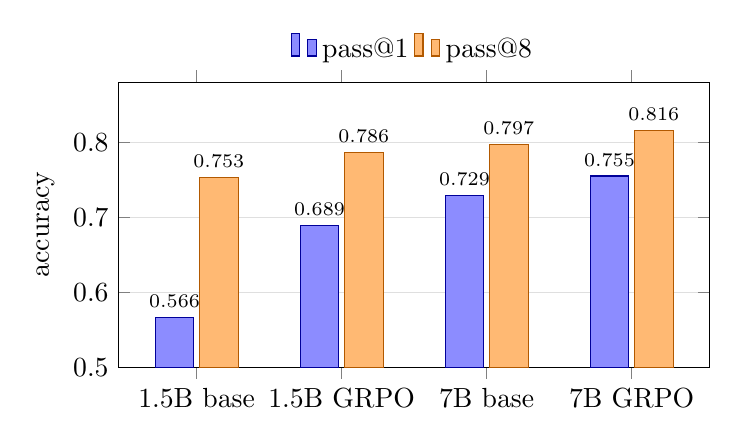
\begin{tikzpicture}
\begin{axis}[
  ybar, bar width=14pt, width=0.75\linewidth, height=5.2cm,
  symbolic x coords={1.5B base,1.5B GRPO,7B base,7B GRPO},
  xtick=data, ymin=0.5, ymax=0.88, ylabel={accuracy},
  legend style={at={(0.5,1.03)},anchor=south,legend columns=2,draw=none,fill=none},
  enlarge x limits=0.18, ymajorgrids, grid style={gray!25},
  nodes near coords, every node near coord/.append style={font=\scriptsize},
  nodes near coords style={/pgf/number format/fixed,/pgf/number format/precision=3}
]
\addplot[fill=blue!45,draw=blue!60!black] coordinates
  {(1.5B base,\PlotPassOneSB) (1.5B GRPO,\PlotPassOneSR) (7B base,\PlotPassOneLB) (7B GRPO,\PlotPassOneLR)};
\addplot[fill=orange!55,draw=orange!70!black] coordinates
  {(1.5B base,\PlotPassEightSB) (1.5B GRPO,\PlotPassEightSR) (7B base,\PlotPassEightLB) (7B GRPO,\PlotPassEightLR)};
\legend{pass@1, pass@8}
\end{axis}
\end{tikzpicture}
\caption{pass@1 rises much more than pass@8, and the rise is largest where the
gap between them was largest.}
\label{fig:passk}
\end{figure}

In both models pass@1 rises more than pass@8 (Table~\ref{tab:headroom},
Figure~\ref{fig:passk}), and the EX gain closely matches the pass@1 gain. Most of
the improvement is turning questions the model sometimes solved into questions
it solves on the first try. The model with more of these questions available
(1.5B) gains more.

This is not shown to be pure sharpening: pass@8 also rises at both scales.
Whether the 1.5B learns set operations it could not do before is measured by
the set-op row of Table~\ref{tab:main}. With two models and one seed, we read
Table~\ref{tab:headroom} as consistent with ``gain scales with headroom,'' not
as evidence for it.

\subsection{Where the model moves: token-level divergence}

We teacher-force the gold query through each base and GRPO model and compute,
per token, the KL divergence between their next-token distributions, the change
in entropy, and the change in gold-token log-probability. Tokens are tagged by
SQL role (keyword, aggregate, table, column, alias, literal, punctuation).

\begin{itemize}
  \item \textbf{Magnitude.} Mean per-token KL is \KLS{} nats at 1.5B and \KLL{}
        at 7B, a $\KLRatio\times$ difference. GRPO fixes \FixedS{} dev questions at 1.5B
        (wrong before, right after) and \FixedL{} at 7B.
        \todo{report questions broken (right before, wrong after) at each scale}.
  \item \textbf{Shape at 1.5B.} Entropy drops by about \EntS{} nats with no strong
        preference for any token role.
  \item \textbf{Shape at 7B.} On the questions GRPO fixed, KL is concentrated on
        aggregate tokens (\ConcAggL$\times$ their share of tokens) and on
        \texttt{FROM}-clause tokens (\ConcFromL$\times$).
\end{itemize}

One reading is that the 1.5B model is still learning general habits for this
task, while the 7B already has them and only adjusts a few decisions.

\subsection{Surface-form convergence}

\begin{table}[h]
\centering
\caption{Surface style of generated SQL, per query on Spider dev.}
\label{tab:style}
\begin{tabular}{lccccc}
\toprule
 & Gold & 1.5B base & 1.5B GRPO & 7B base & 7B GRPO \\
\midrule
Aliases (\texttt{T1}, \texttt{T2}, \dots) & \AliasGold & \AliasSB & \AliasSR & \AliasLB & \AliasLR \\
Qualified \texttt{table.column}           & \todo{} & \QualSB & \QualSR & \QualLB & \QualLR \\
\texttt{JOIN}                             & \todo{} & \JoinSB & \JoinSR & \todo{} & \todo{} \\
\bottomrule
\end{tabular}
\end{table}

The reward only checks the result set. Even so, GRPO drives the 1.5B model to
drop the alias convention used in Spider's gold queries and to write qualified
\texttt{table.column} references instead, close to how the untrained 7B already
writes. The 7B's style does not change. The 1.5B also uses fewer joins, which
matters because unneeded joins are a common error for this model.
Whether this style shift \emph{causes} part of the gain is tested in E3 and E4
(Section~\ref{sec:next}).

\subsection{False positives and reward hacking}

A binary execution reward on one database pays for coincidentally correct
queries, so a policy could learn to produce them. If it did, the EX $-$ TS gap
should grow during training. It moves by \dGapS{} points at 1.5B and \dGapL{} at
7B (Table~\ref{tab:main}). Within this recipe we see no strong reward hacking,
but the false-positive rate is large enough that it should be reported next to
any execution-accuracy gain.

\subsection{Training dynamics}

A mean of \ZeroStd{} of GRPO groups had zero reward variance
(\texttt{frac\_reward\_zero\_std}): all 8 completions were right, or all were
wrong, so they gave no gradient. Most of the compute went to prompts that were
already solved or still out of reach. This is the case dynamic sampling in DAPO
\citep{yu2025dapo} is designed for.

\subsection{Limitations}

Two model sizes, one seed per configuration, one dataset, one reward. The
headroom observation rests on two points. pass@$k$ uses a looser result
comparison than the evaluators. LoRA limits how far the policy can move, so some
differences between scales could come from LoRA capacity rather than RL itself.

\subsection{Running and next experiments}
\label{sec:next}

\begin{enumerate}
  \item \textbf{E3, is the style shift causal? (running)} Prompt the 1.5B base and
        GRPO models to write with or without aliases, and add execution-voted
        sampling (8 samples, majority vote on result sets, no gold). If forcing the
        base model to write \texttt{table.column} recovers part of the gain, style is
        part of the mechanism. If voting matches GRPO, RL here is mostly selection.
  \item \textbf{E4, which neurons carry the style? (running)} Rank all 250{,}880 MLP
        neurons of the 1.5B by their effect on alias preference, using gradients and
        attribution patching from base to GRPO activations. Steer the top neurons and
        measure EX and alias rate on dev, with random-neuron controls and the
        reverse direction on the GRPO model.
  \item \textbf{Robustness.} Two more seeds at 1.5B, and DAPO at 1.5B to test
        whether removing zero-variance groups changes the outcome.
\end{enumerate}

\bibliographystyle{plainnat}
\bibliography{refs}

\end{document}
